160. \begin{figure}[ht!]
\center{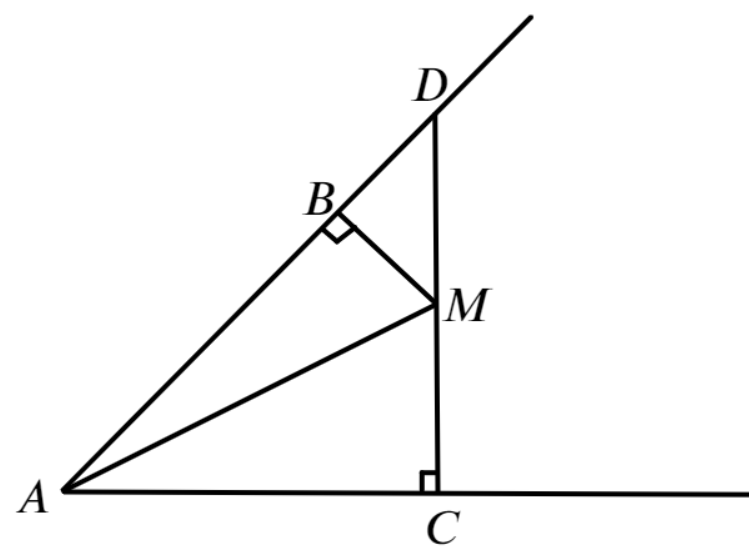
\includegraphics[scale=0.35]{g9-160.png}}
\end{figure}\\
Опустим перпендикуляры $MB$ и $MC$ ($MB=\sqrt{7}$см, $MC=2\sqrt{7}$см) и продлим $MC$ до пересечения с $AB$ в точке $D.$ Найдём $\angle BDM=90^\circ-\angle A=30^\circ,$ тогда $DM=2BM=2\sqrt{7}\text{ см},\ CD=DM+MC=4\sqrt{7}$см и $AC=CD\tg(30^\circ)=\cfrac{4\sqrt{21}}{3}$см. По теореме Пифагора для треугольника $ACM$ получим $AM=\sqrt{\cfrac{112}{3}+28}=\cfrac{14\sqrt{3}}{3}$см.
ewpage
oindent
